%====================================================================%
%                  PIEDRA.TEX                                        %
%====================================================================%

\documentclass{blois}


\bibliographystyle{unsrt}    
% for BibTeX - sorted numerical labels by order of
% first citation.

% A useful Journal macro
\def\Journal#1#2#3#4{{#1} {\bf #2}, #3 (#4)}

% Some useful journal names
\def\NCA{\em Nuovo Cimento}
\def\NIM{\em Nucl. Instrum. Methods}
\def\NIMA{{\em Nucl. Instrum. Methods} A}
\def\NPB{{\em Nucl. Phys.} B}
\def\PLB{{\em Phys. Lett.}  B}
\def\PRL{\em Phys. Rev. Lett.}
\def\PRD{{\em Phys. Rev.} D}
\def\ZPC{{\em Z. Phys.} C}
\def\EPJC{{\em Eur. Phys. J.} C}

% Some other macros used in the sample text
\def\st{\scriptstyle}
\def\sst{\scriptscriptstyle}
\def\mco{\multicolumn}
\def\epp{\epsilon^{\prime}}
\def\vep{\varepsilon}
\def\ra{\rightarrow}
\def\ppg{\pi^+\pi^-\gamma}
\def\vp{{\bf p}}
\def\ko{K^0}
\def\kb{\bar{K^0}}
\def\al{\alpha}
\def\ab{\bar{\alpha}}
\def\be{\begin{equation}}
\def\ee{\end{equation}}
\def\bea{\begin{eqnarray}}
\def\eea{\end{eqnarray}}
\def\CPbar{\hbox{{\rm CP}\hskip-1.80em{/}}}
%temp replacement due to no font
%%%%%%%%%%%%%%%%%%%%%%%%%%%%%%%%%%%%%%%%%%%%%%%%%%
%                                                %
%    BEGINNING OF TEXT                           %
%                                                %
%%%%%%%%%%%%%%%%%%%%%%%%%%%%%%%%%%%%%%%%%%%%%%%%%%

%\newcommand{\Photo}{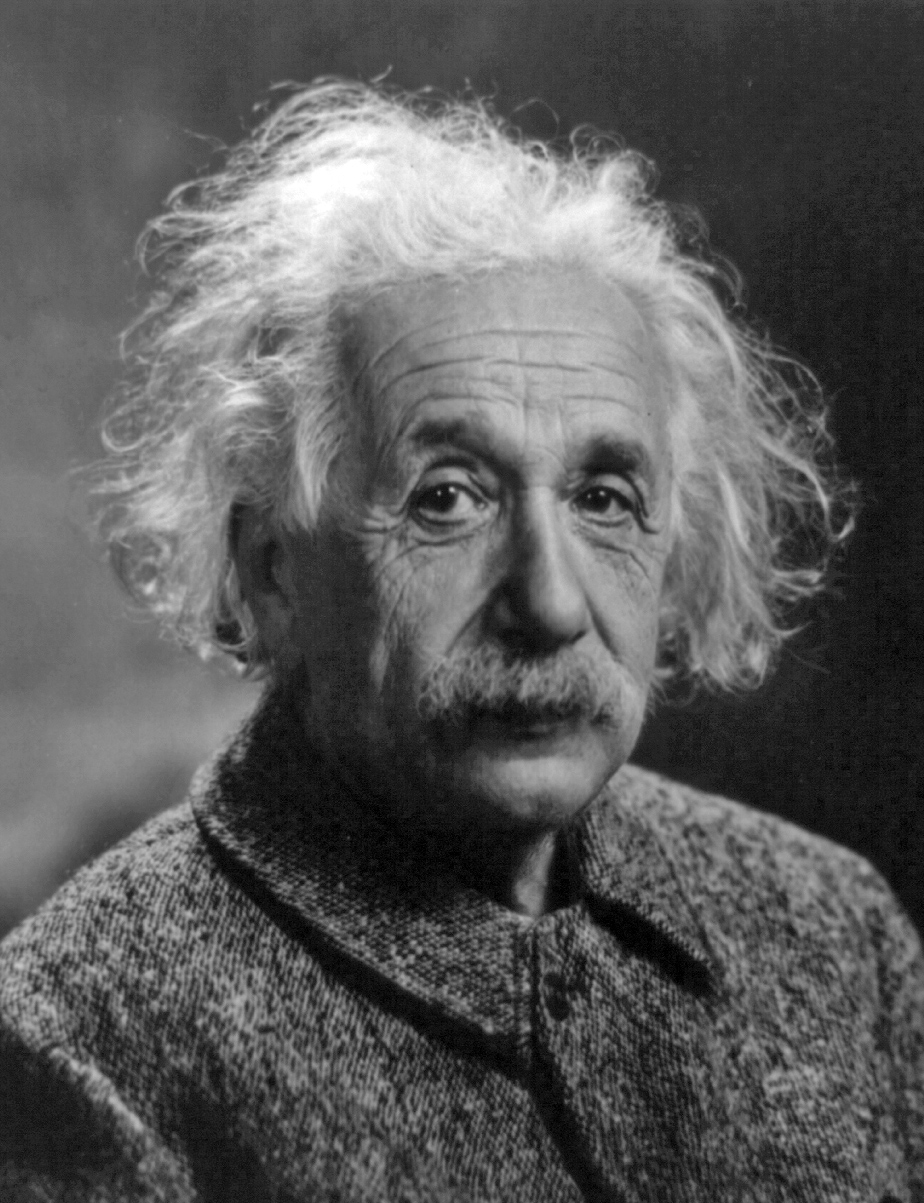
\includegraphics[height=35mm]{mypicture}}
\newcommand{\Photo}{}

\begin{document}
\vspace*{4cm}
\title{Electroweak precision observables ({\boldmath $m_{\rm W}$}, {\boldmath $m_{\rm top}$}) from ATLAS and CMS}


\author{J\'onatan Piedra, for the ATLAS and CMS Collaborations}

\address{Instituto de F\'isica de Cantabria (CSIC - University of Cantabria), Spain}

\maketitle\abstracts{
We present the latest ATLAS and CMS measurements of the top quark mass, the W
boson mass, the effective Electroweak (EW) mixing angle and the on-shell EW
mixing angle. In addition, the uncertainties for current and future measurements
of EW parameters at hadron colliders are investigated.}


%~~~~~~~~~~~~~~~~~~~~~~~~~~~~~~~~~~~~~~~~~~~~~~~~~~~~~~~~~~~~~~~~~~~~~~~~~~~~~~~
\section{Measurement of the forward-backward asymmetry}
%~~~~~~~~~~~~~~~~~~~~~~~~~~~~~~~~~~~~~~~~~~~~~~~~~~~~~~~~~~~~~~~~~~~~~~~~~~~~~~~

The forward-backward asymmetry in electron and muon pairs from ${\rm Z}/\gamma^*$
is measured~\cite{bib:ATLAS-fb-asymmetry} using the 7~TeV pp LHC collision data
recorded with the ATLAS~\cite{bib:ATLAS-detector} detector in 2011 corresponding to an integrated luminosity
of 4.8~${\rm fb}^{-1}$. The data are analysed over a range of dilepton invariant
masses from 66~GeV to 1000~GeV in the central-central electron and muon channels
(pseudorapidity $|\eta| < 2.47$ for the electrons and $|\eta| < 2.4$ for the muons),
and up to 250~GeV in the central-forward electron channel. The latter includes
events where one electron is reconstructed in the forward pseudorapidity range
($2.5 < |\eta| < 4.9$). The forward-backward asymmetry is measured separately
for the three channels as a function of the dilepton invariant mass and unfolded
for detector effects and final-state radiation. The detector level asymmetry
values are used to extract the value of the leptonic effective weak mixing angle,
$\sin^2\theta_{\rm eff}^{\rm lept}$, separately for the three data samples using
a $\chi^2$ minimization method. The results are in good agreement with each other
and with measurements at ${\rm e}^+{\rm e}^-$ colliders, at the Tevatron and by
CMS and LHCb at the LHC, as can be seen in Figure~\ref{fig:theFigure} (left). Results
from the electron and muon final states are combined, yielding
$\sin^2\theta_{\rm eff}^{\rm lept} = 0.2308 \pm 0.0005~({\rm stat.}) \pm 0.0006~({\rm syst.}) \pm 0.0009~({\rm PDF})$.
The dominant uncertainty comes from knowdlege of the PDFs.
%
\begin{figure}
\begin{minipage}{0.40\linewidth}
\centerline{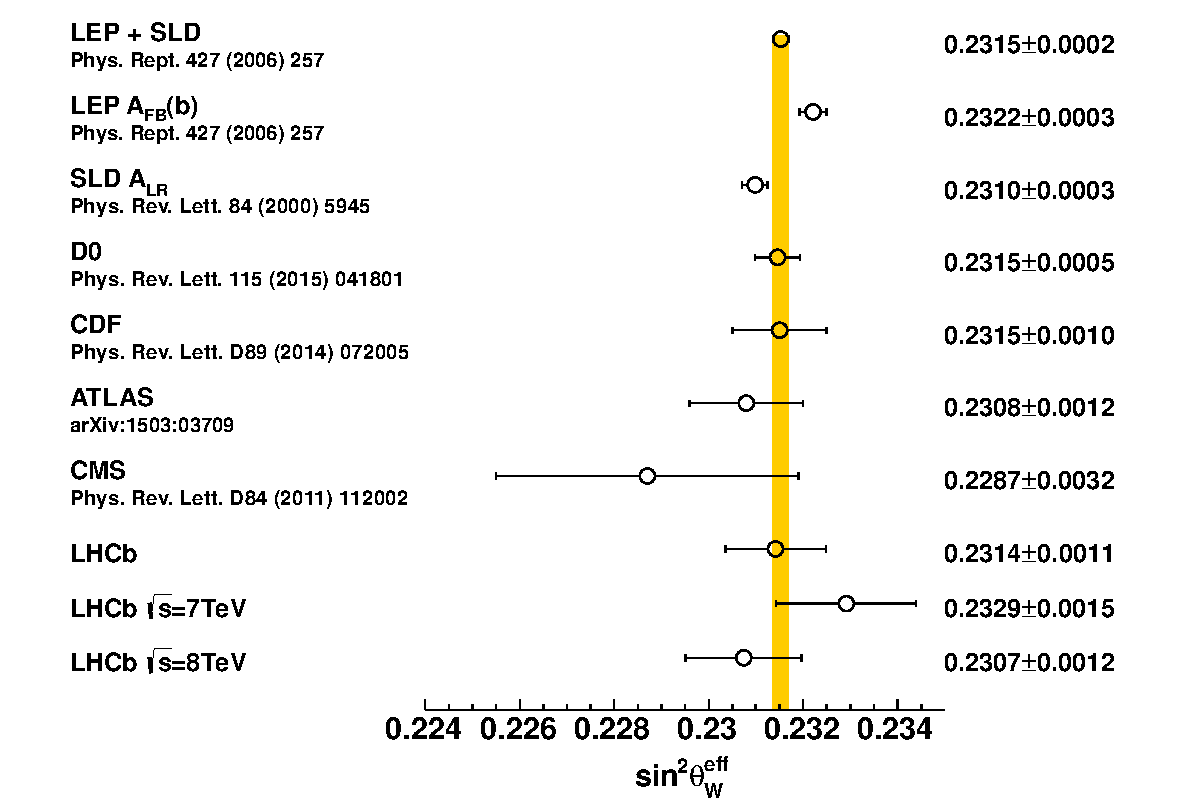
\includegraphics[width=1.00\linewidth]{figures/stw_comp_fullref_final}}
\end{minipage}
%%%\hfill
\begin{minipage}{0.33\linewidth}
\centerline{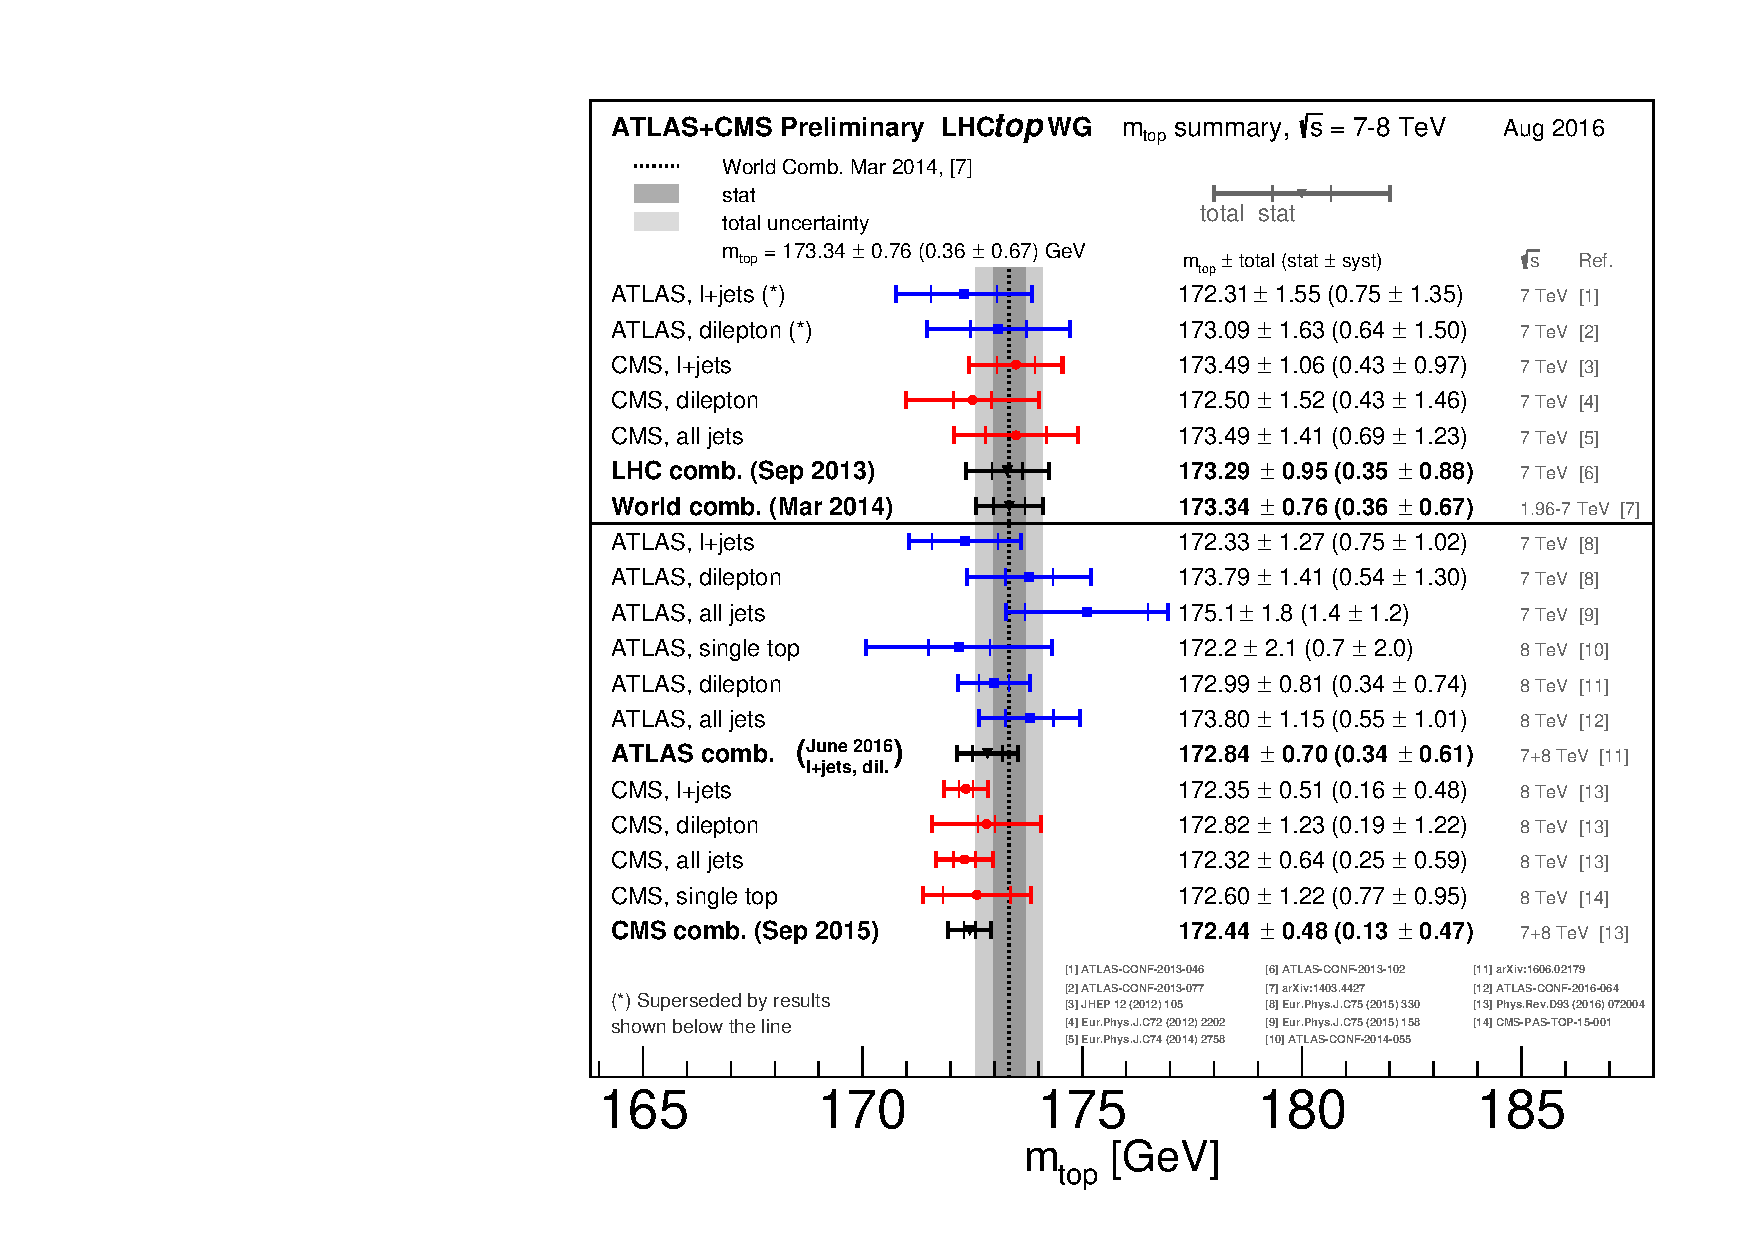
\includegraphics[width=1.00\linewidth]{figures/LHC_topmass_aug2016}}
\end{minipage}
%%%\hfill
\begin{minipage}{0.25\linewidth}
\centerline{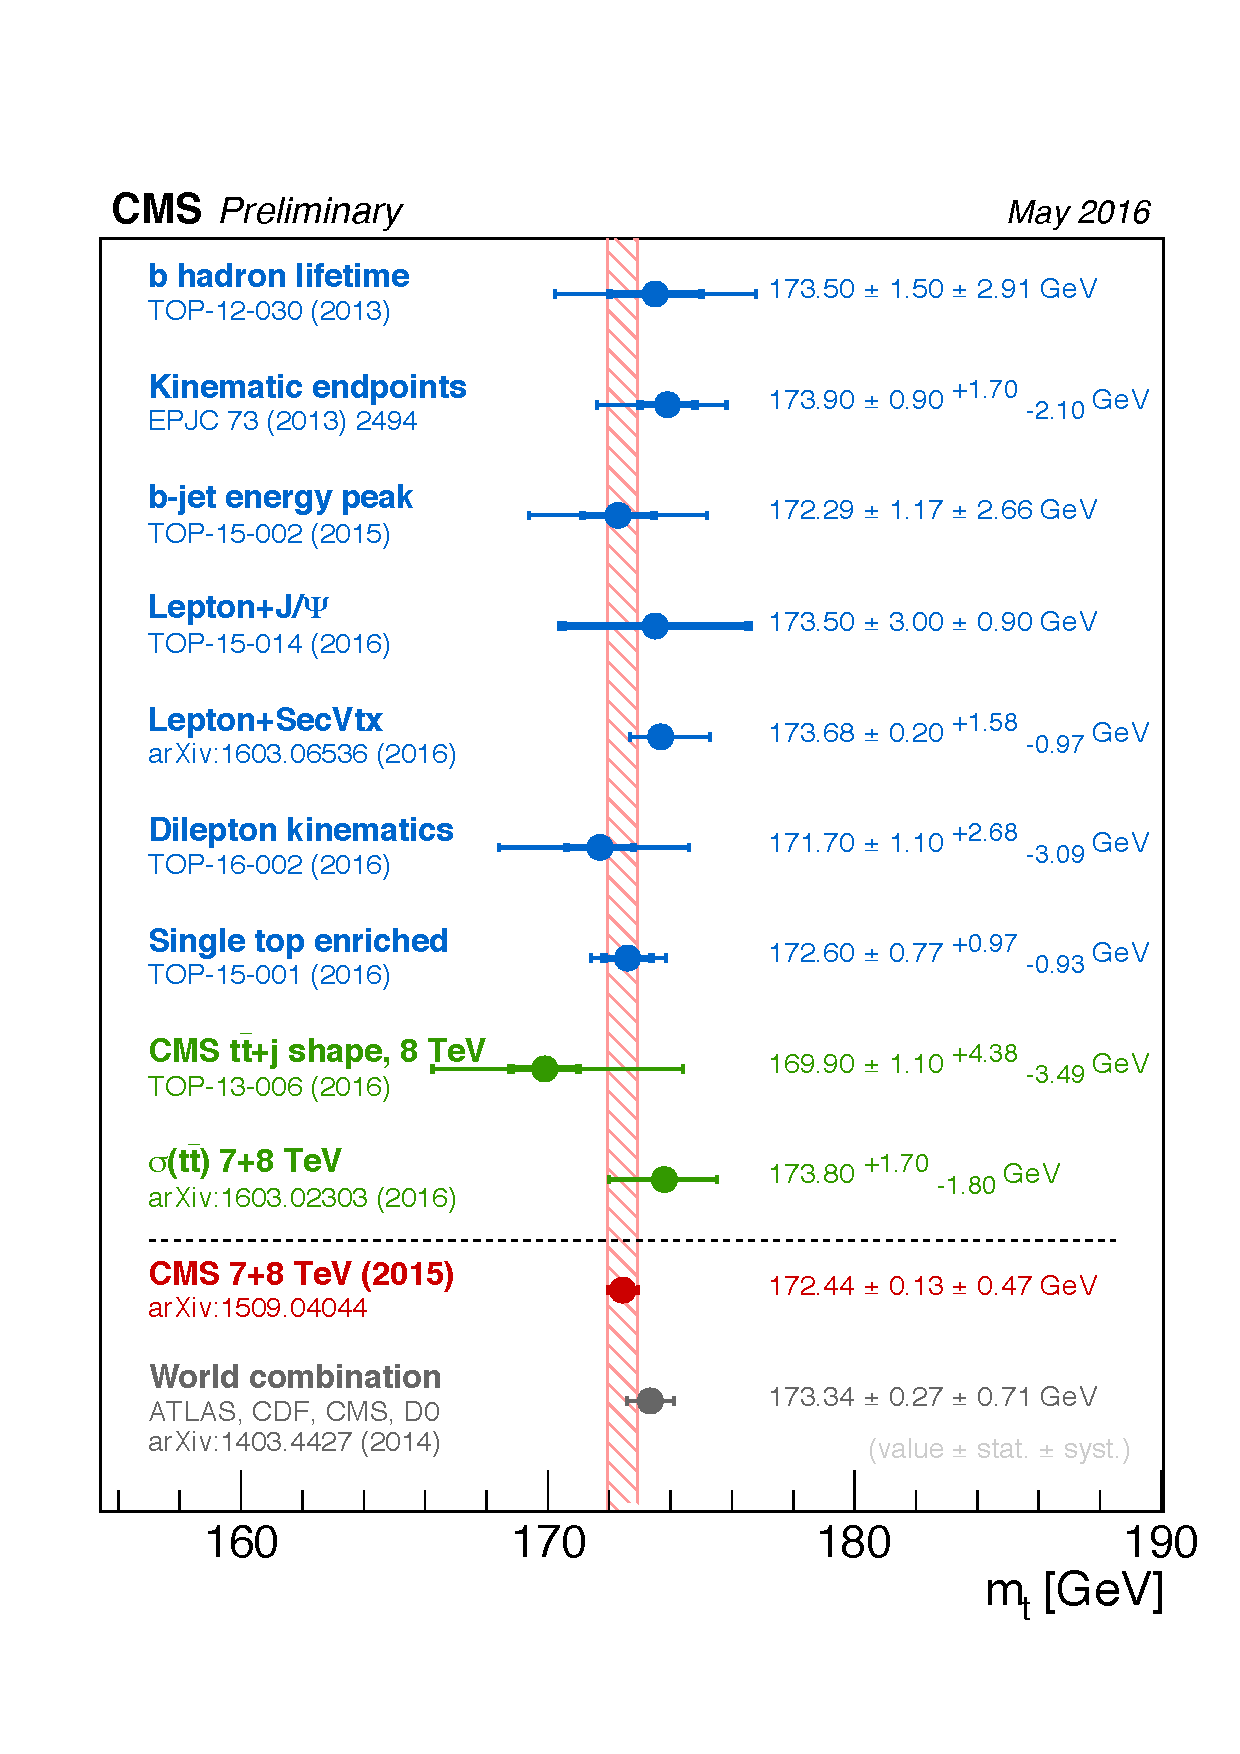
\includegraphics[width=1.00\linewidth]{figures/mtopComb_alt1}}
\end{minipage}
\caption[]{(Left~\cite{bib:LHCb-fb-asymmetry}) Comparison of the $\sin^2\theta_{\rm eff}^{\rm lept}$ results, including
the most precise measurements from LEP, SLD, Tevatron and LHC. The combined LEP and
SLD measurement is indicated by the vertical yellow band.
(Center~\cite{bib:LHCTopWG-topMass}) Summary of the ATLAS and CMS direct $m_{\rm top}$ measurements. The
results are compared with the LHC and Tevatron+LHC $m_{\rm top}$ combinations.
For each measurement, the statistical uncertainty includes the jet scale factor
(JSF) and b-jet scale factor (bJSF) contributions (when applicable), while the
sum of the remaining systematic uncertainties is reported separately. The JSF
and bJSF contributions are statistical in nature and apply to analyses performing
in-situ (top quark pair based) jet energy calibration procedures. The results
below the line are results produced after the LHC and Tevatron+LHC combinations
were performed.
(Right~\cite{bib:CMS-topMassAlternative}) Summary of Run-I CMS alternative $m_{\rm top}$ measurements.}
\label{fig:theFigure}
\end{figure}


%~~~~~~~~~~~~~~~~~~~~~~~~~~~~~~~~~~~~~~~~~~~~~~~~~~~~~~~~~~~~~~~~~~~~~~~~~~~~~~~
\section{W-like measurement of the Z boson mass}
%~~~~~~~~~~~~~~~~~~~~~~~~~~~~~~~~~~~~~~~~~~~~~~~~~~~~~~~~~~~~~~~~~~~~~~~~~~~~~~~

The standard model (SM) quantum corrections to the mass of the W boson, $m_{\rm W}$,
are dominated by contributions dependent on the masses of the top quark,
$m_{\rm top}$, and the Higgs boson, $m_{\rm H}$, as well as the fine-structure
constant $\alpha$. Therefore, combining precise measurements of these three masses
provides a critical test of the nature and consistency of the SM. After the discovery
of the Higgs boson, a global electroweak fit predicts $m_{\rm W} = 80.358 \pm 0.008$~GeV,
a result with an uncertainty smaller than that from the combination of all direct
$m_{\rm W}$ measurements. This means that the mass of the W boson should be
measured with a precision of 6~MeV or better, to be compared with the 15~MeV
uncertainty of the current $m_{\rm W}$ world average. The analysis presented
here by CMS~\cite{bib:CMS-detector,bib:CMS-WlikeZmass} constitutes a milestone towards a high
precision W mass measurement with
${\rm W\to\mu\nu}$ events. The study is made on the basis of a dimuon data sample
collected by CMS at 7~TeV, corresponding to an integrated luminosity of
$4.7~{\rm fb}^{-1}$. The muon momentum scale calibration has been improved by
correcting the curvature of the muon tracks for small variations of the magnetic
field, in addition of residual misalignment effects, and imperfect modelling of
the material resulting in different energy loss. This calibration has been done
with the $J/\psi$ and $\Upsilon(1S)$ resonances, and a closure test has been
performed with Z+jets events, achieving a precision below 8~MeV. In addition,
the hadronic recoil of the events has also been calibrated, achieving
a precision good enough to pursue an accurate measurement of the W mass
at the LHC, even in the presence of multiple interactions. As a proof of principle
the analysis technique has been used to measure the mass of the Z boson after
removing one of its decay muons, getting a result compatible with the
world-average value.


%~~~~~~~~~~~~~~~~~~~~~~~~~~~~~~~~~~~~~~~~~~~~~~~~~~~~~~~~~~~~~~~~~~~~~~~~~~~~~~~
\section{Top mass}
%~~~~~~~~~~~~~~~~~~~~~~~~~~~~~~~~~~~~~~~~~~~~~~~~~~~~~~~~~~~~~~~~~~~~~~~~~~~~~~~

The mass of the top quark is an important parameter of the SM, and precise
measurements provide critical inputs to fits of global electroweak parameters
that, as mentioned in the previous section, help assess the internal consistency
of the SM. In addition, the value of $m_{\rm top}$ affects the stability of the
SM Higgs potential, which has cosmological implications.


%~~~~~~~~~~~~~~~~~~~~~~~~~~~~~~~~~~~~~~~~~~~~~~~~~~~~~~~~~~~~~~~~~~~~~~~~~~~~~~~
\subsection{Direct measurements}
%~~~~~~~~~~~~~~~~~~~~~~~~~~~~~~~~~~~~~~~~~~~~~~~~~~~~~~~~~~~~~~~~~~~~~~~~~~~~~~~

In the ATLAS paper~\cite{bib:ATLAS-topMass7TeV} the top quark mass has been
measured via a three-dimensional template method in the ${\rm t{\bar t}\to \rm lepton+jets}$
final state, and using a one-dimensional template in the ${\rm t{\bar t}\to dilepton}$
channel. Both analyses are based on 7~TeV pp collision data
corresponding to an integrated luminosity of $4.6~{\rm fb^{-1}}$.
In the lepton+jets analysis $m_{\rm top}$ is determined together with a global
jet energy scale factor and a residual b-to-light jet energy scale factor. A
combination of the lepton+jets and dilepton results is performed using the BLUE
technique, exploiting the full uncertainty breakdown, and taking into account the
correlation of the measurements for all sources of the systematic uncertainty.
The result is $m_{\rm top} = 172.99 \pm 0.48~({\rm stat.}) \pm 0.78~({\rm syst.})$~GeV.
The total uncertainty of the combination corresponds to 0.91~GeV and is currently
dominated by systematic uncertainties due to jet calibration and modelling of the
${\rm t{\bar t}}$ events. In the ATLAS paper~\cite{bib:ATLAS-topMassDilepton8TeV}
the top quark mass is measured in the ${\rm t{\bar t}\to dilepton}$ channel from
about $20.2~{\rm fb}^{-1}$ of 8 TeV proton-proton collision data recorded by the
ATLAS detector at the LHC. Compared to the latest ATLAS measurement in this decay
channel, the event selection is refined exploiting the average transverse
momentum $p_{\rm T}$ of the lepton-b-jet pairs to enhance the fraction of
correctly reconstructed events, thereby reducing the systematic uncertainties.
Using the optimal point in terms of total uncertainty observed in a phase-space
scan of this variable as an additional event selection criterion, the measured
value of $m_{\rm top}$ is $172.99\pm 0.41~({\rm stat.})\pm 0.74~({\rm syst.})$~GeV,
with a total uncertainty of 0.84~GeV. The precision is mainly limited by systematic
uncertainties, mostly by the calibration of the jet energy scale. This measurement
is combined with the aforementioned ATLAS results in the lepton+jets and dilepton
channels from 7~TeV data. Using a dedicated mapping of uncertainty categories, the
combination of the three measurements results in
$m_{\rm top} = 172.84 \pm 0.34~({\rm stat.}) \pm 0.61~({\rm syst.})$~GeV, with a
total uncertainty of 0.70~GeV, which means a relative precision of 0.4\%. The
result is mostly limited by the calibration of the jet energy scales and by the
Monte Carlo modelling of signal events.

A new set of measurements of the top quark mass has been also presented by
CMS~\cite{bib:CMS-topMass8TeV}, based on the data recorded at 8 TeV during 2012,
and corresponding to a luminosity of
$19.7~{\rm fb}^{-1}$. The top quark mass has been measured in the lepton+jets,
all-jets and dilepton decay channels, giving values of
$172.35 \pm 0.16~({\rm stat.}) \pm 0.48~({\rm syst.})$~GeV,
$172.32 \pm 0.25~({\rm stat.}) \pm 0.59~({\rm syst.})$~GeV, and
$172.82 \pm 0.19~({\rm stat.}) \pm 1.22~({\rm syst.})$~GeV, respectively.
Individually, these constitute the most precise measurements in each of the
decay channels studied. When combined with the published CMS results at 7 TeV,
a top quark mass measurement of
$172.44 \pm 0.13~({\rm stat.}) \pm 0.47~({\rm syst.})$~GeV is obtained. This is
the most precise measurement of $m_{\rm top}$ to date, with a total uncertainty
of 0.48~GeV. These measurements use analysis techniques in which either
$m_{\rm top}$ alone is determined or $m_{\rm top}$ and the overall jet energy
scale factor are determined simultaneously. For the lepton+jets and the all-jets
channels analyses have been based on the ideogram technique, which is a joint
maximum likelihood fit that determines the top quark mass and the overall jet
energy scale factor.
While the ideogram technique provides the most precise measurements, it is not
suitable for dilepton events where the presence of more than one neutrino
introduces uncertainties in the use of the measured missing transverse energy.
Instead, for the dilepton channel, the analytical matrix weighting technique
has been used.
The top quark mass has also been studied as a function of the event
kinematical properties in the lepton+jets channel. No indication of a kinematical
bias in the measurement is observed and the data are consistent with a range of
predictions from current theoretical models of ${\rm t{\bar t}}$ production.
Both ATLAS and CMS latest $m_{\rm top}$ direct measurements are summarized
in Figure~\ref{fig:theFigure} (center).


%~~~~~~~~~~~~~~~~~~~~~~~~~~~~~~~~~~~~~~~~~~~~~~~~~~~~~~~~~~~~~~~~~~~~~~~~~~~~~~~
\subsection{Alternative measurements}
%~~~~~~~~~~~~~~~~~~~~~~~~~~~~~~~~~~~~~~~~~~~~~~~~~~~~~~~~~~~~~~~~~~~~~~~~~~~~~~~

In contrast to the ${\rm t{\bar t}}$ production via the strong
interaction, in pp collisions at the LHC, top quarks can also be produced singly
via the weak charged-current interactions, giving another possibility for
measuring $m_{\rm top}$. In the ATLAS document~\cite{bib:ATLAS-singleTop8TeV}
we present the first measurement of the top quark mass in a phase-space
dominated by single top quarks produced via the weak interaction. The signal
corresponds to a mix of topologies containing single top quarks produced in the
$t$-channel and of ${\rm t{\bar t}}$ pairs, for which the total background
fraction has been reduced to below 30\% using a neural network based discriminant.
Candidate events are selected in the lepton + missing
energy + 2-jet channel, with exactly one of the jets required to be b-tagged,
from $20.3~{\rm fb}^{-1}$ of 8~TeV data.
The measured $m_{\rm top}$ in the combined electron and muon channels is
$172.2 \pm 0.7~({\rm stat.}) \pm 2.0~({\rm syst.})$~GeV, in good agreement
with the measurements performed in ${\rm t{\bar t}}$ events. In a similar way,
in the CMS document~\cite{bib:CMS-singleTop8TeV} the top quark mass is
measured on $19.7~{\rm fb}^{-1}$ of data collected at 8~TeV. The top quark is
reconstructed from its decay ${\rm t\to W^+b}$, with the W boson decaying
leptonically in the muon channel. Specific event topology and kinematic 
properties are used in order to enrich the sample in single top quark events
in the $t$-channel, at the expense of top-quark pair production events. A fit
to the reconstructed top invariant mass distribution yields
$m_{\rm top} = 172.60 \pm 0.77~({\rm stat.}) \pm 0.97~({\rm syst.})$~GeV.

The top quark mass can also be measured from the inclusive cross section for
${\rm t{\bar t}}$ production. With this method the top quark mass scheme is
unambiguously defined in the theoretical calculations, albeit it is less precise,
due to a relatively weak sensitivity of the inclusive cross section to the
top quark mass, as well as to the large uncertainties on the factorization and
normalization scales and the proton PDF. In these
ATLAS~\cite{bib:ATLAS-topPoleMass} and CMS~\cite{bib:CMS-topPoleMass} documents,
$m_{\rm top}$ is extracted from a measurement of the normalized differential
cross section for ${\rm t{\bar t}}$ production with at least one additional
jet, as a function of the inverse of the invariant mass of the
${\rm t{\bar t}}$ + 1-jet system. This distribution is sensitive to
$m_{\rm top}$ because the amount of gluon radiation depends on its value,
with large effects in the phase-space region relatively close to the
${\rm t{\bar t}}$ + 1-jet production threshold. ATLAS uses $4.6~{\rm fb}^{-1}$ of
7 TeV pp collision data. By looking at the lepton+jets channel with two
b-tagged jets, the measured top quark pole mass is
$173.7 \pm 1.5~({\rm stat.}) \pm 1.4~({\rm syst.})^{+1.0}_{-0.5}~({\rm theory})$~GeV.
CMS uses $19.7~{\rm fb}^{-1}$ of 8 TeV data. By looking at the dileptonic decay
channels the measured top quark pole mass is
$169.9 \pm 1.1~({\rm stat.})^{+2.5}_{-3.1}~({\rm syst.})^{+3.6}_{-1.6}~({\rm theory})$~GeV.

In the ATLAS document~\cite{bib:ATLAS-topCrossSection} the inclusive ${\rm t{\bar t}}$
production cross-section has been measured using $4.6~{\rm fb}^{-1}$ at 7~TeV and
$20.3~{\rm fb}^{-1}$ at 8~TeV, in the ${\rm e}\mu$ decay channel with one and two
b-tagged jets.
This result has been used to determine the top quark pole mass via the dependence
of the predicted cross-section on $m_{\rm top}^{\rm pole}$, giving a value of
$172.9^{+2.5}_{-2.6}$~GeV. The same is done in the following CMS
paper~\cite{bib:CMS-topCrossSection}, using $5.0~{\rm fb}^{-1}$ at 7 TeV and
$19.7~{\rm fb}^{-1}$ at 8~TeV. Looking also at the ${\rm e}\mu$ decay channel,
CMS measures $m_{\rm top}^{\rm pole} = 173.8^{+1.7}_{-1.8}$~GeV. This is the
most precise result found by CMS, when using the NNPDF3.0 PDF set.

In the CMS document~\cite{bib:CMS-topMassFromJpsi} the top quark mass is extracted
from a simultanoeus template fit to the invariant mass of the leading
lepton-$J/\psi$ candidate, in a sample enriched in top decays with
${\rm b}\to J/\psi + {\rm X}\to \mu^+\mu^- + {\rm X}$. This sample corresponds
to $19.7~{\rm fb}^{-1}$ pp collisions at 8~TeV. The method provides a top quark
mass measurement of $173.5 \pm 3.0~({\rm stat.}) \pm 0.9~({\rm syst.})$~GeV.
A similar study has been presented by CMS~\cite{bib:CMS-topMassFromCharged} where
the top quark mass is measured using only the kinematic properties of its charged
decay products, showing minimal sensitivity to experimental sources of uncertainty.
This result, together with all alternative top mass measurements, can be found in
Figure~\ref{fig:theFigure} (right). Finally, in the CMS
document~\cite{bib:CMS-topMassFromLeptons} a novel technique for measuring the
top quark mass using only leptonic observables is discussed, by analyzing top
quark pair events with one electron, one muon and at least one jet in the final
state, sleected from $19.7~{\rm fb}^{-1}$ of 8~TeV pp data. The transverse
momentum distribution of the charged lepton pair is chosen to extract the
following top mass,
$171.7 \pm 1.1~({\rm stat.}) \pm 0.5~({\rm exp.})^{+2.5}_{-3.1}~({\rm theory})^{+0.8}_{-0.0}~(p_{\rm T})$~GeV.


%~~~~~~~~~~~~~~~~~~~~~~~~~~~~~~~~~~~~~~~~~~~~~~~~~~~~~~~~~~~~~~~~~~~~~~~~~~~~~~~
\section*{References}
%~~~~~~~~~~~~~~~~~~~~~~~~~~~~~~~~~~~~~~~~~~~~~~~~~~~~~~~~~~~~~~~~~~~~~~~~~~~~~~~

\begin{thebibliography}{99}

\bibitem{bib:ATLAS-fb-asymmetry}ATLAS Collaboration, \Journal{JHEP}{09}{049}{2015}.

\bibitem{bib:ATLAS-detector}ATLAS Collaboration, \Journal{JINST}{3}{S08003}{2008}.

\bibitem{bib:CMS-detector}CMS Collaboration, \Journal{JINST}{3}{S08004}{2008}.

\bibitem{bib:CMS-WlikeZmass}CMS Collaboration, CMS-SMP-14-007 (2016).

\bibitem{bib:LHCb-fb-asymmetry}LHCb Collaboration, \Journal{JHEP}{1511}{190}{2015}.

\bibitem{bib:LHCTopWG-topMass}https://twiki.cern.ch/twiki/bin/view/LHCPhysics/LHCTopWGSummaryPlots.

\bibitem{bib:CMS-topMassAlternative}https://twiki.cern.ch/twiki/bin/view/CMSPublic/PhysicsResultsTOPSummaryFigures.

\bibitem{bib:ATLAS-topMass7TeV}ATLAS Collaboration, \Journal{\EPJC}{75}{330}{2015}.

\bibitem{bib:ATLAS-topMassDilepton8TeV}ATLAS Collaboration, \Journal{\PLB}{761}{350-371}{2016}.

\bibitem{bib:CMS-topMass8TeV}CMS Collaboration, \Journal{\PRD}{93}{072004}{2016}.

\bibitem{bib:ATLAS-singleTop8TeV}ATLAS Collaboration, ATLAS-CONF-2014-055 (2014).

\bibitem{bib:CMS-singleTop8TeV}CMS Collaboration, CMS-TOP-15-001 (2016).

\bibitem{bib:ATLAS-topPoleMass}ATLAS Collaboration, \Journal{JHEP}{10}{121}{2015}.

\bibitem{bib:CMS-topPoleMass}CMS Collaboration, CMS-TOP-13-006 (2016).

\bibitem{bib:ATLAS-topCrossSection}ATLAS Collaboration, \Journal{\EPJC}{74}{3109}{2014}.

\bibitem{bib:CMS-topCrossSection}CMS Collaboration, \Journal{JHEP}{08}{029}{2016}.

\bibitem{bib:CMS-topMassFromJpsi}CMS Collaboration, CMS-TOP-15-014 (2016).

\bibitem{bib:CMS-topMassFromCharged}CMS Collaboration, \Journal{PRD}{93}{092006}{2016}.

\bibitem{bib:CMS-topMassFromLeptons}CMS Collaboration, CMS-TOP-16-002 (2016).

\end{thebibliography}

\end{document}

%%%%%%%%%%%%%%%%%%%%%
% End of piedra.tex %
%%%%%%%%%%%%%%%%%%%%%
